\documentclass[,a4paper,12pt]{article}
\usepackage[utf8]{inputenc}
\usepackage[siunitx]{circuitikz}
\usepackage{graphicx}
\usepackage{multirow}
\usepackage{float}
\usepackage{makecell} % Pakiet do łamania wierszy w tabeli
\usepackage[table]{xcolor}
\usepackage{cellspace}
\setlength{\cellspacetoplimit}{4pt} % Górny padding
\setlength{\cellspacebottomlimit}{4pt} % Dolny padding
\usepackage{array}
\usepackage{amsmath}
% Odstępy w tabelach
\setlength{\tabcolsep}{8pt} % Poziome odstępy
\renewcommand{\arraystretch}{1.5} % Pionowe odstępy
\newenvironment{conditions}
  {\par\vspace{\abovedisplayskip}\noindent\begin{tabular}{>{$}l<{$} @{${}={}$} l}}
  {\end{tabular}\par\vspace{\belowdisplayskip}}
\usepackage[T1]{fontenc}
\usepackage[MEX]{polski}
\usepackage{booktabs}
\usepackage[usenames,dvipsnames]{xcolor}
\usepackage{geometry}
\usepackage{siunitx} % Dodanie pakietu siunitx do formatowania jednostek
\sisetup{separate-uncertainty, output-decimal-marker = {,}}
\geometry{a4paper, total={170mm,257mm}, left=20mm, top=20mm}
\usepackage{indentfirst} % Dodaje wcięcia po sekcjach
\setlength{\parindent}{1em} % Ustawia globalne wcięcia w akapitach
\renewcommand{\footnotesize}{\fontsize{10pt}{12pt}}
%\renewcommand{\thesection}{\Roman{section}}
\usepackage[backend=biber,style=numeric, sorting=none]{biblatex}
\addbibresource{bibliografia.bib} % Wskaż plik .bib z wpisami bibliograficznymi
\usepackage{biblatex}
\renewcommand{\cite}{\supercite}
\usepackage{titlesec}
\titlespacing*{\paragraph}{0pt}{1.5ex plus 1ex minus .2ex}{1.5ex plus 1ex minus .2ex}
\titleformat{\paragraph}[block]{\normalfont\normalsize\bfseries}{\theparagraph}{1em}{}
\usepackage[pdfusetitle]{hyperref}
\hypersetup{
    pdfauthor={Inez Małecka},
    pdftitle={Sprawozdanie laboratoryjne}, 
    pdfsubject={Praca wykonana samodzielnie, jestem jedynym autorem.}, 
    pdfkeywords={potencjometr, prawo Ohma, raport, laboratorium}, 
}



\begin{document}
\begin{center}
    \begin{tabular}{|p{6cm}|p{4.5cm}|p{4.5cm}|}
        \hline
        \multicolumn{3}{|c|}{\textbf{\large ELEKTRONIKA I ELEKTROTECHNIKA}} \\ 

        \multicolumn{3}{|c|}{\textbf{ Laboratorium}} \\
        \hline
        \multicolumn{3}{|l|}{Temat ćwiczenia: Właściwości Potencjometru, Zastosowanie prawa Ohma} \\
        \hline
        {\small Ćwiczenie wykonali:} &
        {\small Numer ćwiczenia:} &
        {\small Prowadzący:} \\
        \begin{center}
            \textbf{Inez Małecka (52738) \\ Igor Miszczak (52742) \\ Oliwia Organista-Michalak (52755)}
        \end{center} &
        \begin{center}
            \textbf{Lab01}
        \end{center} &
        \begin{center}
            \textbf{Mgr inż. Leszek Kędzierski}
        \end{center}
        \\
        \hline
        {\small Sprawozdanie opracowali:} &
        {\small Data wykonania ćwiczenia:} &
        {\small Ocena:} \\
        \begin{center}
            \textbf{
        Inez Małecka (52738) \\ Igor Miszczak (52742) \\ Oliwia Organista-Michalak (52755)}
        \end{center}
         &
         \begin{center}
             \textbf{04/01/2025}
         \end{center}
        &
        \\
        \hline
    \end{tabular}
\end{center}

\section{{\textsc{Wprowadzenie}}}
Celem niniejszego ćwiczenia było zapoznanie z budową podstawowych układów elektrycznych, zrozumienie sposób ich połączeń oraz opanowanie prawidłowej obsługi sprzętu laboratoryjnego wykorzystywanego w trakcie prac w laboratorium. W trakcie zajęć dokonano eksperymentalnego omówienia prawa Ohma, doświadczalne zapoznanie się z działaniem potencjometru wraz z uwzględnieniem analizy wyników zwracając szczególną uwagę na błędy pomiarowe oraz ich potencjalne pochodzenie.\\\par

Pojęcie prądu elektrycznego definiowane jest jako uporządkowany przepływ ładunków elektrycznych w postaci elektronów bądź jonów w przestrzeni lub przewodniku. Definiować go także można jako całkowitą prędkość przepływu ładunku elektrycznego przez powierzchnię\cite{walker2014}. Podstawowymi wielkościami w standardzie SI używanymi do opisu prądu elektrycznego są:
\begin{itemize}
    \item \textbf{Natężenie prądu}\\
    Natężenie prądu elektrycznego $I$ definiuje się jako stosunek ładunku elektrycznego, który przepływa przez poprzeczny przekrój przewodnika do czasu przepływu tego ładunku $t$.\\ 
    \begin{equation}
        I=\frac{dq}{dt}\quad[A]
    \end{equation}
    Natężenie prądu określić można również przez ilość ładunków przepływających przez powierzchnię z prędkością $v$ przez powierzchnię $S$ gdzie $n$ określa koncentrację ładunków\cite{bolkowski1986}.
    \begin{equation}
        I=qnvS\quad [A]
    \end{equation}
    \item \textbf{Napięcie prądu}\\
    Napięcie elektryczne to stosunek pracy wykonanej przeciwko polu, podczas przenoszenia ładunku elektrycznego między punktami, dla których określa się napięcie, do wartości tego ładunku\cite{bolkowski1986}.
    \begin{equation}
        U_{AB}=\varphi B - \varphi A = \frac{W_{A\rightarrow B}}{q}\quad[V]
    \end{equation}
    \item \textbf{Rezystancja}\\
    Rezystancja elektryczna, jest wielkością charakteryzującą relację między napięciem a natężeniem prądu elektrycznego przepływającego przez przewodnik w obwodzie prądu stałego. Rezystencję oznacza się literą $R$, jednakże jej jednostką jest Ohm [$\Omega$]. Należy zauważyć iż prawo Ohma nie należy do uniwersalnych praw przyrody, jest jedynie właściwością konkretnej klasy materiałów w ograniczonym zakresie gęstości prądów.
    \begin{equation}
        R = \frac{U}{I}\quad[\Omega]
    \end{equation}
\end{itemize}\par
Mimo faktu iż prawo Ohma znajduje swoje zastosowanie jedynie dla wąskiej gamy materiałów oraz ograniczonego zakresu gęstości prądów, opisanie go stanowiło ważny moment w historii fizyki, a tym samym w rozwoju elektroniki. Opisanie rezystencji umożliwiło również stworzenie pojęcia przewodnictwa elektrycznego - odwrotności rezystencji. Rezystencja, a tym samym przewodnictwo zależne jest od pewnej gamy czynników: materiału, stanu, temperatury, oraz długości i grubości.\\ \par
Rezystory są jednymi z podstawowych elementów pasywnych w obwodach elektronicznych. Ich głównym zadaniem jest ograniczanie przepływu prądu elektrycznego oraz regulowanie napięcia w obwodzie. Zasadnicza część rezystora (opornika) zbudowana jest z materiału o małej przewodności elektrycznej, a z obwodem zewnętrznym łączy się za pośrednictwem dwóch dobrze przewodzących wyprowadzeń\cite{platt2021}.\\ \par
Potencjometr, znany również jako rezystor o zmiennej wartości, to specyficzny typ rezystora, który umożliwia regulację napięcia. Dzięki tej właściwości potencjometr często znajduje zastosowanie jako narzędzie do redukcji napięcia. Jest powszechnie używany w układach sterujących czułością wejść, równoważeniem kanałów wyjściowych w systemach wzmacniaczy oraz w obwodach regulujących pracę różnych czujników, takich jak detektory ruchu. Potencjometr jest również wykorzystywany w sytuacjach, gdzie konieczna jest dynamiczna zmiana wartości rezystancji. Urządzenie to wyposażone jest w trzy wyprowadzenia. Dwa skrajne są połączone z końcami wewnętrznego elementu rezystancyjnego, zazwyczaj wykonanego z materiału przewodzącego, określanego jako ścieżka. Trzecie, centralne wyprowadzenie, jest podłączone do ruchomego styku, zwanego ślizgaczem, który porusza się po ścieżce. Sterowanie ślizgaczem odbywa się poprzez obracanie osi potencjometru lub przesuwanie suwaka. Podłączenie napięcia zasilającego do skrajnych wyprowadzeń powoduje, że napięcie odbierane przez ślizgacz zmienia się w zależności od jego położenia na ścieżce. W takim układzie potencjometr działa na zasadzie dzielnika napięcia rezystancyjnego\cite{platt2021}.
\section{\textsc{Przebieg ćwiczenia}}
\subsection{\textsc{Ćwiczenie 1-2 "Własności Potencjometru"}}
Ćwiczenie wykonano na module edukacyjnym \texttt{KL-24001} o numerze seryjnym \texttt{208288-2021.10} oraz przy użyciu miernika uniwersalnego \texttt{UT58C} o numerze seryjnym \texttt{0089004}.\\ \par
W celu poprawnego zapoznania się z działaniem rezystora zmiennego - potencjometru, wykonano następujące kroki:
\begin{enumerate}
    \item Posługując się miernikiem uniwersalnym \texttt{UT58C} ustawionym w tryb pomiaru rezystencji (funkcja omomierza), dokonano pomiarów rezystancji między wyprowadzeniami \texttt{1} oraz \texttt{3} potencjometru \texttt{VR1} znajdującego się na makiecie edukacyjnej \texttt{KL-24001}. Zmierzoną rezystancję, po ustabilizowaniu wyniku na wyświetlaczu urządzenia pomiarowego zapisano w protokole, zmierzona wartość wynosiła:
    \begin{equation}
        R_{13} = 5,31\hspace{5pt}k\Omega
    \end{equation}
\item Po zmierzeniu rezystancji $R_{13}$, stale obserwując wskazania
    miernika uniwersalnego, przekręcono powolnym ruchem pokrętło
    potencjometru w prawo aż do osiągnięcia punktu granicznego. W
    granicznej prawej pozycji pokrętła potencjometru, nie zaobserwowano zmiany wartości mierzonej rezystancji opornika \texttt{VR1}.
\item Następnie, w analogiczny sposób dokonano pomiaru wartości
    rezystancji przy pokrętle przekręcanym w lewą stronę. Również, przez całą drogę ruchu pokrętła, jak i w granicznej jego pozycji nie zaobserwowano zmiany wartości mierzonej rezystancji.
    \begin{figure}[H]
\begin{center}
\begin{circuitikz}[american]
\draw
(5,0) to
  (5,3) to [rmeterwa, t=$\Omega$, a = 5.31k$\Omega$] (-1,3) --
  (-1,0) -- (1,0) to [pR, l = pokrętło, a = \texttt{VR1}] (3,0) -- (5,0)
(1,0) node[below] {$1$} % Wyjście 1
  (3,0) node[below] {$3$} % Wyjście 3
;
\end{circuitikz} \\ 
\caption{Schemat układu połączonego na wyjściach \texttt{1} oraz \texttt{3}}\end{center}\end{figure} 
\label{fig:1-2-1}
\item Przepięto sondy pomiarowe miernika uniwersalnego \texttt{UT58C} na wyprowadzenia \texttt{2} oraz \texttt{3} potencjometru \texttt{VR1}. Następnie, monitorując w sposób ciągły wartości wyświetlane na ekranie miernika uniwersalnego przekręcono pokrętło potencjometru do granicznej lewej wartości i zapisano zmierzoną rezystencję w protokole, wynosiła ona:
\begin{equation}
    R_{23}=5,31\hspace{5pt}k\Omega
\end{equation}
\item Po zanotowaniu ustabilizowanego wyniku, całą operację powtórzono, przekręcając pokrętło potencjometru w prawą stronę, cały czas monitorując wartości wyświetlane na ekranie miernika uniwersalnego. Po ustabilizowaniu wyniku zapisano jego wartość w protokole laboratoryjnym, rezystencja w granicznej prawej pozycji wynosiła:
\begin{equation}
    R_{23}=5,7\hspace{5pt}\Omega
\end{equation}
\begin{figure}[H]
\begin{center}
\begin{circuitikz}[american]
\draw
(5,0) to
  (5,3) to [rmeterwa, t=$\Omega$, a = 5.7$\Omega$ - 5.31k$\Omega$] (-1,3) --
  (-1,0) -- (1,0) to [pR, l = pokrętło, a = \texttt{VR1}] (3,0) -- (5,0)
(1,0) node[below] {$2$} % Wyjście 1
  (3,0) node[below] {$3$} % Wyjście 3
;
\end{circuitikz} \\ 
\caption{Schemat układu połączonego na wyjściach \texttt{2} oraz \texttt{3}}\end{center}\end{figure} 
\label{fig:1-2-2}
\item Przepięto sondy miernika uniwersalnego na wyprowadzenia \texttt{1} oraz \texttt{2} potencjometru \texttt{VR1}.
\item Monitorując w sposób ciągły wartości wyświetlane na ekranie miernika uniwersalnego przekręcono pokrętło potencjometru do granicznej lewej wartości i zapisano zmierzoną rezystencję w protokole, wynosiła ona:
\begin{equation}
    R_{12}=5,5\hspace{5pt}\Omega
\end{equation}
\item Po zanotowaniu ustabilizowanego wyniku, całą operację powtórzono, przekręcając pokrętło potencjometru w prawą stronę, cały czas monitorując wartości wyświetlane na ekranie miernika uniwersalnego. Po ustabilizowaniu wyniku zapisano jego wartość w protokole laboratoryjnym, rezystencja w granicznej prawej pozycji wynosiła:
\begin{equation}
    R_{12}=5,31\hspace{5pt}k\Omega
\end{equation}
\begin{figure}[H]
\begin{center}
\begin{circuitikz}[american]
\draw
(5,0) to
  (5,3) to [rmeterwa, t=$\Omega$, a = 5.5$\Omega$ - 5.31k$\Omega$] (-1,3) --
  (-1,0) -- (1,0) to [pR, l = pokrętło, a = \texttt{VR1}] (3,0) -- (5,0)
(1,0) node[below] {$1$} % Wyjście 1
  (3,0) node[below] {$2$} % Wyjście 3
;
\end{circuitikz} \\ 
\caption{Schemat układu połączonego na wyjściach \texttt{1} oraz \texttt{2}}\end{center}\end{figure} 
\label{fig:1-2-3}
\item Po wykonaniu powyższych kroków, przekręcono gałkę potencjometru całkowicie w lewo i rozpoczęto doświadczenie mające na celu sprawdzenie zależności rezystancji na wyjściach potencjometru. Na granicznej pozycji, połączono diody miernika z wyjściami \texttt{1,2} a następnie bez zmiany wartości potencjometru z wyjściami \texttt{2,3}. Analogicznie pomiary przeprowadzono dla $\frac{1}{4}$ , $\frac{1}{2}$ oraz $\frac{3}{4}$ obrotu pokrętła, oraz granicznego wychylenia pokrętła w prawo, a dane zapisano w tabeli poniżej.

\begin{table}[H]
    \centering
    \begin{tabular}{lccc}
    \hline
    Pozycja osi potencjometru & $R_{12}$ & $R_{23}$ & $R_{12}+R_{23}$ \\ \hline
    Całkowicie w lewo & $5,50\hspace{5pt}\Omega$ & $5,31\hspace{5pt}k\Omega$ & $5,316\hspace{5pt}k\Omega$   \\
    $\frac{1}{4}$ obrotu & $1,19\hspace{5pt}k\Omega$ & $4,17\hspace{5pt}k\Omega$ & $5,360\hspace{5pt}k\Omega$   \\
    $\frac{1}{2}$ obrotu & $2,61\hspace{5pt}k\Omega$ & $2,79\hspace{5pt}k\Omega$ & $5,400\hspace{5pt}k\Omega$   \\
    $\frac{3}{4}$ obrotu & $4,26\hspace{5pt}k\Omega$ & $1,12\hspace{5pt}k\Omega$ & $5,380\hspace{5pt}k\Omega$   \\
    Całkowicie w prawo & $5,31\hspace{5pt}k\Omega$ & $5,70\hspace{5pt}\Omega$ & $5,316\hspace{5pt}k\Omega$ \\ \hline 
    \end{tabular}
    \caption{Wyniki pomiaru rezystancji potencjometru}
    \label{tab:Tabela1}
\end{table}
Przykładowy sposób obliczenia sumy rezystancji $R_{12}+R_{23}$ przedstawiono w równaniu~\eqref{eq:r12r23}.
\end{enumerate}
\subsection{\textsc{Ćwiczenie 1-5 "Zastosowanie prawa Ohma"}}
Ćwiczenie wykonano na module edukacyjnym \texttt{KL-24001} o numerze seryjnym \texttt{208288-2021.10}, module edukacyjnym \texttt{KL-24002} o numerze seryjnym \texttt{208274-2021.10}, module edukacyjnym \texttt{KL-22001} oraz przy użyciu miernika uniwersalnego \texttt{UT58C} o numerze seryjnym \texttt{0089004}.\\ \par
W celu eksperymentalnego określenia prawa Ohma, wykonano następujące kroki:
\begin{enumerate}
    \item Posługując się miernikiem uniwersalnym \texttt{UT58C} zmierzono opór rezystora $R_1$ umieszczonego na makiecie \texttt{KL-24002}. Po ustabilizowaniu wyniku na wyświetlaczu miernika uniwersalnego, wynik zapisano w raporcie. Rezystancja w/w opornika wynosiła:
    \begin{equation}
        R_1=0,991\hspace{5pt}k\Omega
        \label{er1}
    \end{equation}
    \item Następnie, przed rozpoczęciem konstruowania układu doświadczalnego, miernik uniwersalny w trybie pomiaru napięcia (tryb woltomierza) połączona do wyprowadzeń plusa (\texttt{V+}) oraz masy (\texttt{GND2}) zasilacza o regulowanym napięciu wyjściowym, umieszczonym na module \texttt{KL-22001}, zgodnie ze schematem~\ref{fig:1-5-1}. Na tak ustawionym układzie, odczytując wskazania urządzenia pomiarowego, regulowano napięcie na zasilaczu aż do osiągnięcia napięcia wyjściowego równego: \begin{equation}
        U=+10,0 \hspace{5pt}V
        \label{fał1}
    \end{equation}
    
        \begin{figure}[H] \begin{center} \begin{circuitikz}[american]
        \draw
        (5,0) to
        (5,3) to [rmeterwa, t=$V$, v = 10.0$V$] (-1,3) --
        (-1,0) -- (1,0) to [dcisource] (3,0) -- (5,0)
        (0.75,0) node[below] {GND2} % Wyjście 1
        (3,0) node[below] {V+} % Wyjście 3
        ;
        \end{circuitikz} \\ 
        \caption{Schemat układu dla nastawy napięcia na zasilaczu} \label{fig:1-5-1}
        \end{center}\end{figure} 
    \item  Po nastawieniu napięcia na zasilaczu, urządzenie pomiarowe (miernik uniwersalny) odłączono, oraz przygotowano układ doświadczalny jak wskazano na schemacie~\ref{fig:1-5-2}. Na połączonym do układu miliamperomierzu odczytano wynik pomiaru prądu w układzie: 
    \begin{equation}
        I_{rzeczywiste}=9,0\hspace{5pt}mA    
    \end{equation}
    \begin{figure}[H] \begin{center} \begin{circuitikz}[american]
        \draw
        (5,0) to[R=$0.991\Omega$] (5,3) 
        to [rmeterwa, t= $mA$, a=$9.0mA$] (-1,3)
        to [short] (-1,0)
        to [dcisource] (5,0)
        (0.75,0) node[below] {GND2} % Wyjście 1
        (3,0) node[below] {V+} % Wyjście 3
        ;
        \end{circuitikz} \\ 
        \caption{Schemat układu dla nastawy napięcia na zasilaczu} \label{fig:1-5-2}
        \end{center}\end{figure} 
    \item Wykorzystując wcześniej zmierzoną doświadczalnie rezystancję opornika $R_1$ (Równanie~\ref{er1}) oraz stałą nastawę napięcia podawaną na układ (Równanie~\ref{fał1}), obliczono teorytyczną wartość natężenia prądu w układzie eksperymentalnym. Zaobserwowano znaczną różnicę między natężeniem zmierzonym a obliczonym. Napięcie obliczono wzorem na prawo Ohma (Równanie~\ref{Iteoryt1}) i wynosiło ono:
    \begin{equation}
        I_{teorytyczne} = 10,090\hspace{10pt}mA
    \end{equation}
    \item Następnie zwiększono napięcie w układzie, tak by urządzenie pomiarowe wpięte w układ doświadczalny (miliamperomierz) wskazywał wartość:
    \begin{equation}
        I_2 = 9,0\hspace{5pt}mA
        \label{noweNaterzenie}
    \end{equation}
    \item Na podstawie nowej wartości natężenia prądu (Równanie~\ref{noweNaterzenie}) oraz znanej rezystancji opornika $R_1$ (Równanie~\ref{er1}) znajdującego się w układzie obliczono (Równanie~\ref{Vteoryt1}) teoretyczne napięcie w układzie:
    \begin{equation}
        U_{teorytyczne}=14,865\hspace{5pt}V
    \end{equation}
    \item W dalszym ciągu doświadczenia odłączono układ doświadczalny od źródła prądu stałego, na jego miejsce połączono miernik uniwersalny w trybie miernika napięcia (woltomierz) analogicznie jak przedstawiono na Rysunku~\ref{fig:1-5-1}. Za jego pomocą zmierzono realne napięcie dostarczane do układu doświadczalnego:
    \begin{equation}
        U_{rzeczywiste}=15,48\hspace{5pt}V
    \end{equation}
    \item Na tak ustawionym układzie, odczytując wskazania urządzenia pomiarowego, regulowano napięcie na zasilaczu aż do osiągnięcia napięcia wyjściowego równego: \begin{equation}
        U=+15,0 \hspace{5pt}V
        \label{fał2}
    \end{equation}
    \item W następnym kroku ćwiczenia, do układu przedstawionego na Rysunku~\ref{fig:1-5-2} dodatkowo podpięto wyprowadzenia \texttt{1} i \texttt{2} potencjometru \texttt{VR1} z makiety edukacyjnej \texttt{24001} zgodnie ze schematem~\ref{fig:1-5-3} przedstawionym poniżej.
    \begin{figure}[H] \begin{center} \begin{circuitikz}[american]
        \draw
        (5,0) to[R=$R_1$] (5,3) 
        to [pR, a = \texttt{VR1} ] (-1,3)
        to [rmeterwa, t= $mA$,] (-1,0)
        to [dcisource] (5,0)
        (3,3) to [short] (3,2.25) to [short] (2,2.25) to [short] (2,2.5)
        
        (0.75,0) node[below] {GND2} % Wyjście 1
        (3,0) node[below] {V+} % Wyjście 3
        ;
        \end{circuitikz} \\ 
        \caption{Schemat układu dla nastawy napięcia na zasilaczu} \label{fig:1-5-3}
        \end{center}\end{figure} 
        \item W tak przygotowanym układzie doświadczalnym, za pomocą pokrętła potencjometru, zmieniano wartość jego rezystancji aż do osiągnięcia wskazania miliamperomierza równej:
        \begin{equation}
            I_{zmierzone}=5,0\hspace{5pt}mA
            \label{newNaterzenie}
        \end{equation}
        \item Posługując się prawem Ohma obliczono teoretyczną rezystancję dla potencjometru \texttt{VR1} (Równanie~\ref{Rteoryt}). Wynosiła ona:
        \begin{equation}
            R_{VR1\,teorytyczne}=2,009\hspace{10pt}k\Omega
        \end{equation}
        \item Następnie posługując się omomierzem zmierzono realny opór potencjometru w układzie:
        \begin{equation}
            R_{VR1}=1,666\hspace{10pt}k\Omega
        \end{equation}

    
\end{enumerate}










\section{\textsc{Obliczenia i interpretacja wyników}}
\subsection{\textsc{Obliczenie sumy $R_{12}+R_{23}$}}
Obliczenie całkowitej rezystancji potencjometru na przykładzie pierwszego wiersza Tabeli~\ref{tab:Tabela1}:
\begin{equation}
R_{\text{całkowita}} = R_{12} + R_{23} = 5,50\,\Omega + 5310\,\Omega = 5315,5\,\Omega \approx 5,316\,k\Omega
\label{eq:r12r23}
\end{equation}
\subsection{\textsc{Obliczenie teoretycznego natężenia prądu w układzie}}
\begin{equation}
    I_{teorytyczne}=\frac{U}{R_1}=\frac{10\,V}{991\,\Omega}=0,01009082\,A= 10,091\,mA
    \label{Iteoryt1}
\end{equation}
\subsection{\textsc{Obliczenie teoretycznego napięcia prądu w układzie}}
\begin{equation}
    U_{teorytyczne}=RI = 991\,\Omega\,\times\,0,015\,A = 14,865\,V
    \label{Vteoryt1}
\end{equation}
\subsection{\textsc{Obliczenie teoretycznej rezystencji opornika w układzie}}
\begin{equation}
    R_{VR1}+R_1=\frac{U}{I} \Longrightarrow R_{VR1}=\frac{U}{I}-R_1 = \frac{15,0V}{0,005A}-0,991\Omega=3,0\Omega-0,991\Omega=2,009\Omega 
    \label{Rteoryt}
\end{equation}
\subsection{\textsc{Błąd wewnętrzny przyrządów pomiarowych}}
W eksperymencie skorzystano z dwóch urządzeń pomiarowych - miernika laboratoryjnego \texttt{UT58C} oraz miliamperomierza wbudowanego w makietę edukacyjną \texttt{KL-22001}. Oba te urządzenia obarczone są pewnym błędem pomiarowym który to też został opisany przez producenta w instrukcji obsługi sprzętu laboratoryjnego.\\ \par Z instrukcji dla sprzętu \texttt{UT58C} wynika że dla zakresu wartości pomiarów dokonanych na ćwiczeniach, błąd pomiarowy wynosił "$\pm\hspace{5pt}0,5\%$ wskazania $\pm$ 5 cyfr" dla pomiaru napięcia prądu, "$\pm\hspace{5pt}0,8\%$ wskazania $\pm$ 3 cyfry" dla pomiarów rezystancji do $200\Omega$, oraz  "$\pm\hspace{5pt}0,8\%$ wskazania $\pm$ 1 cyfra"  dla reszty pomiarów rezystancji w trakcie ćwiczenia\cite{instrukcja_ut58}.\\ \par Z instrukcji dla makiety \texttt{KL-22001} wynika że dla zakresu wartości pomiarów dokonanych na ćwiczeniach, błąd pomiarowy wynosił "$\pm\hspace{5pt}0,5\%$ wskazania + 1 cyfra" dla pomiaru natężenia prądu przy pomocy wbudowanego amperomierza\cite{ndn_instrukcja_736}. \\ \par
Oznacza to że przy porównaniu obliczonych wartości teoretycznych z wartościami rzeczywistymi brać pod uwagę musimy także błąd pomiarowy wartości podstawianych do obliczeń oraz błąd pomiarowy wartości porównywanych. W przypadku obliczania błędu wartości obliczonej na podstawie dwóch wartości o różnych błędach pomiarowych, stosujemy zasadę propagacji błędów, zgodnie z którą:
\begin{equation}
    \frac{\Delta Z}{Z}=\frac{\Delta A}{A} + \frac{\Delta B}{B}
\end{equation}
gdzie:
\begin{conditions}
    Z&$A\times B,\ lub\ Z=\frac{A}{B}$
\end{conditions}
\subsubsection{Propagacja błędów dla wartości teoretycznych}

\paragraph{1. Propagacja błędów dla teoretycznego natężenia prądu:}
Z równania (\ref{Iteoryt1}) mamy:
\[
I_{\text{teoretyczne}} = \frac{U}{R_1}
\]
Propagacja błędów dla dzielenia wynosi:
\[
\frac{\Delta I}{I} = \frac{\Delta U}{U} + \frac{\Delta R_1}{R_1}
\]
Podstawiając wartości:
\[
\Delta U = \pm (0,5\% \times 10 \, \text{V} + 5 \times 0,1 \, \text{V}) = \pm 0,55 \, \text{V}
\]
\[
\Delta R_1 = \pm (0,8\% \times 991 \, \Omega + 1 \times 0,1 \, \Omega) = \pm 7,928 \, \Omega
\]
\[
\frac{\Delta I}{I} = \frac{0,55}{10} + \frac{7,928}{991} = 0,055 + 0,008 = 0,063
\]
Stąd:
\[
\Delta I = 0,063 \times 0,01009082 \, \text{A} \approx 0,000635 \, \text{A} = 0,635 \, \text{mA}
\]
Ostatecznie:
\[
I_{\text{teoretyczne}} = 10,091 \, \text{mA} \pm 0,635 \, \text{mA}
\]

\paragraph{2. Propagacja błędów dla teoretycznego napięcia:}
Z równania (\ref{Vteoryt1}) mamy:
\[
U_{\text{teoretyczne}} = R_1 \times I
\]
Propagacja błędów dla mnożenia wynosi:
\[
\frac{\Delta U}{U} = \frac{\Delta R_1}{R_1} + \frac{\Delta I}{I}
\]
Podstawiając wartości:
\[
\Delta R_1 = \pm 7,928 \, \Omega, \quad R_1 = 991 \, \Omega, \quad \Delta I = \pm 0,001 \, \text{A}, \quad I = 0,015 \, \text{A}
\]
\[
\frac{\Delta U}{U} = \frac{7,928}{991} + \frac{0,001}{0,015} = 0,008 + 0,067 = 0,075
\]
\[
\Delta U = 0,075 \times 14,865 \, \text{V} \approx 1,115 \, \text{V}
\]
Ostatecznie:
\[
U_{\text{teoretyczne}} = 14,865 \, \text{V} \pm 1,115 \, \text{V}
\]

\paragraph{3. Propagacja błędów dla teoretycznej rezystancji:}
Z równania (\ref{Rteoryt}) mamy:
\[
R_{VR1} = \frac{U}{I} - R_1
\]
Propagacja błędów dla ilorazu i różnicy wynosi:
\[
\frac{\Delta R_{VR1}}{R_{VR1}} = \frac{\Delta U}{U} + \frac{\Delta I}{I}
\]
Podstawiając wartości:
\[
\Delta U = \pm 0,55 \, \text{V}, \quad U = 15,0 \, \text{V}, \quad \Delta I = \pm 0,001 \, \text{A}, \quad I = 0,005 \, \text{A}
\]
\[
\frac{\Delta R_{VR1}}{R_{VR1}} = \frac{0,55}{15} + \frac{0,001}{0,005} = 0,037 + 0,2 = 0,237
\]
\[
\Delta R_{VR1} = 0,237 \times 2,009 \, \Omega \approx 0,475 \, \Omega
\]
Ostatecznie:
\[
R_{VR1} = 2,009 \, \Omega \pm 0,475 \, \Omega
\]
\subsubsection{\textsc{Obliczenie błędów dla wartości rzeczywistych (zmierzonych)}}

\paragraph{1. Błąd zmierzonego natężenia prądu:}
Dla miliamperomierza wbudowanego w makietę \texttt{KL-22001}, błąd wynosi:
\[
\Delta I = \pm (0,5\% \times I_{\text{rzeczywiste}} + 1 \, \text{cyfra})
\]
Podstawiając \( I_{\text{rzeczywiste}} = 9,0 \, \text{mA} \) oraz rozdzielczość \( 1 \, \text{cyfra} = 0,1 \, \text{mA} \):
\[
\Delta I = \pm (0,005 \times 9,0 + 0,1) = \pm (0,045 + 0,1) = \pm 0,145 \, \text{mA}
\]
Ostatecznie:
\[
I_{\text{rzeczywiste}} = 9,0 \, \text{mA} \pm 0,145 \, \text{mA}
\]

\paragraph{2. Błąd zmierzonego napięcia:}
Dla miernika \texttt{UT58C}, błąd pomiaru napięcia wynosi:
\[
\Delta U = \pm (0,5\% \times U_{\text{rzeczywiste}} + 5 \, \text{cyfr})
\]
Podstawiając \( U_{\text{rzeczywiste}} = 15,48 \, \text{V} \) oraz rozdzielczość \( 1 \, \text{cyfra} = 0,1 \, \text{V} \):
\[
\Delta U = \pm (0,005 \times 15,48 + 5 \times 0,1) = \pm (0,0774 + 0,5) = \pm 0,5774 \, \text{V}
\]
Zaokrąglając:
\[
U_{\text{rzeczywiste}} = 15,48 \, \text{V} \pm 0,578 \, \text{V}
\]

\paragraph{3. Błąd zmierzonej rezystancji potencjometru:}
Dla miernika \texttt{UT58C}, błąd pomiaru rezystancji w zakresie do \( 200 \, \Omega \) wynosi:
\[
\Delta R = \pm (0,8\% \times R_{\text{rzeczywiste}} + 3 \, \text{cyfry})
\]
Podstawiając \( R_{\text{rzeczywiste}} = 1,666 \, \text{k}\Omega = 1666 \, \Omega \) oraz rozdzielczość \( 1 \, \text{cyfra} = 0,1 \, \Omega \):
\[
\Delta R = \pm (0,008 \times 1666 + 3 \times 0,1) = \pm (13,328 + 0,3) = \pm 13,628 \, \Omega
\]
Zaokrąglając:
\[
R_{\text{rzeczywiste}} = 1,666 \, \text{k}\Omega \pm 13,63 \, \Omega
\]
\subsubsection{\textsc{Porównanie zakresu możliwego wyniku teoretycznego z możliwym wynikiem rzeczywistym}}
\paragraph{1. Natężenie prądu:}
Dla teoretycznego natężenia prądu (\(I_{\text{teoretyczne}} = 10,091 \, \text{mA} \pm 0,635 \, \text{mA}\)) oraz rzeczywistego (\(I_{\text{rzeczywiste}} = 9,0 \, \text{mA} \pm 0,145 \, \text{mA}\)), zakresy wynoszą:
\[
I_{\text{teoretyczne}} \in \langle 9,456 \, \text{mA}, 10,726 \, \text{mA} \rangle
\]
\[
I_{\text{rzeczywiste}} \in \langle 8,855 \, \text{mA}, 9,145 \, \text{mA} \rangle
\]
Zakresy te nie nakładają się.

\paragraph{2. Napięcie:}
Dla teoretycznego napięcia (\(U_{\text{teoretyczne}} = 14,865 \, \text{V} \pm 1,115 \, \text{V}\)) oraz rzeczywistego (\(U_{\text{rzeczywiste}} = 15,48 \, \text{V} \pm 0,578 \, \text{V}\)), zakresy wynoszą:
\[
U_{\text{teoretyczne}} \in \langle 13,750 \, \text{V}, 15,980 \, \text{V} \rangle
\]
\[
U_{\text{rzeczywiste}} \in \langle 14,902 \, \text{V}, 16,058 \, \text{V} \rangle
\]
Zakresy te częściowo się pokrywają.

\paragraph{3. Rezystancja potencjometru:}
Dla teoretycznej rezystancji potencjometru (\(R_{\text{VR1 teoretyczne}} = 2,009 \, \text{k}\Omega \pm 0,475 \, \text{k}\Omega\)) oraz rzeczywistej (\(R_{\text{VR1 rzeczywiste}} = 1,666 \, \text{k}\Omega \pm 0,01363 \, \text{k}\Omega\)), zakresy wynoszą:
\[
R_{\text{VR1 teoretyczne}} \in \langle 1,534 \, \text{k}\Omega, 2,484 \, \text{k}\Omega \rangle
\]
\[
R_{\text{VR1 rzeczywiste}} \in \langle 1,652 \, \text{k}\Omega, 1,680 \, \text{k}\Omega \rangle
\]
Zakresy te częściowo się pokrywają.
\section{\textsc{Wnioski}}
W trakcie ćwiczeń ugruntowano wiedzę na temat prawa Ohma, oraz podstawowych praw fizycznych na których bazują podstawowe układy elektryczne. W trakcie analizy zabranych i obliczonych wyników, zaobserwowano jak istotne dla analizy statystycznej jest branie pod uwagę błędów wynikających z niedokładności ludzkiej, niedokładności sprzętu pomiarowego, jak i czynników środowiskowych niezależnych od laboranta.
\begin{itemize}
    \item Badanie charakterystyki potencjometru wykazało, że zmiana rezystancji pomiędzy jego wyprowadzeniami przebiegała zgodnie z założeniami teoretycznymi. Suma rezystancji pomiędzy wyprowadzeniami w granicznych punktach pokrętła odpowiadała całkowitej rezystancji potencjometru, co potwierdziło poprawność działania tego elementu. Ewentualne niedokładności pomiarowe nie powinny wynikać z niedokładności pomiarowej sprzętu labolatoryjnego - w trakcie prowadzenia eksperymentu środowisko nie uległo zmianie, nie zmieniła się osoba prowadząca pomiary czy ich metodyka, uważa się że na różnice w wartościach rezystancji przy pokrętłach przekręconych na pozycję $\frac{1}{4}$,  $\frac{1}{2}$ czy $\frac{3}{4}$, bezpośredni wpływ miał brak podziałki (skali) przy pokrętle potencjometru co prowadziło do ustawienia pokrętła nie równo z założoną odległością od punktu granicznego.
    \item Wyniki obliczeń teoretycznych dla natężenia prądu oraz napięcia w układzie w większości przypadków mieściły się w zakresie wyników rzeczywistych uwzględniających błędy pomiarowe. Wyjątek stanowiły niektóre pomiary natężenia prądu, w których zauważono różnicę wynikającą z błędów eksperymentalnych, takich jak nieidealne połączenia w obwodzie lub ograniczenia przyrządów pomiarowych. Analiza propagacji błędów pomiarowych pozwoliła na określenie ich wpływu na wyniki. Zarówno miernik uniwersalny (\texttt{UT58C}), jak i miliamperomierz wbudowany w makietę edukacyjną wprowadzały niepewność do wyników. Uwzględnienie błędów pomiarowych umożliwiło lepszą interpretację wyników i ich pewien zakres zgodności z teorią.
    \item Wyniki pokazały, że dokładność użytych przyrządów pomiarowych ma istotny wpływ na uzyskiwane wyniki. Nawet niewielkie niepewności wprowadzane przez urządzenia mogą prowadzić do zauważalnych różnic w rezultatach, szczególnie w obliczeniach wymagających propagacji błędów.
\end{itemize}
\section{\textsc{Bibliografia}}
\printbibliography[heading=none]
\section{\textsc{Protokół z zajęć}}\par
    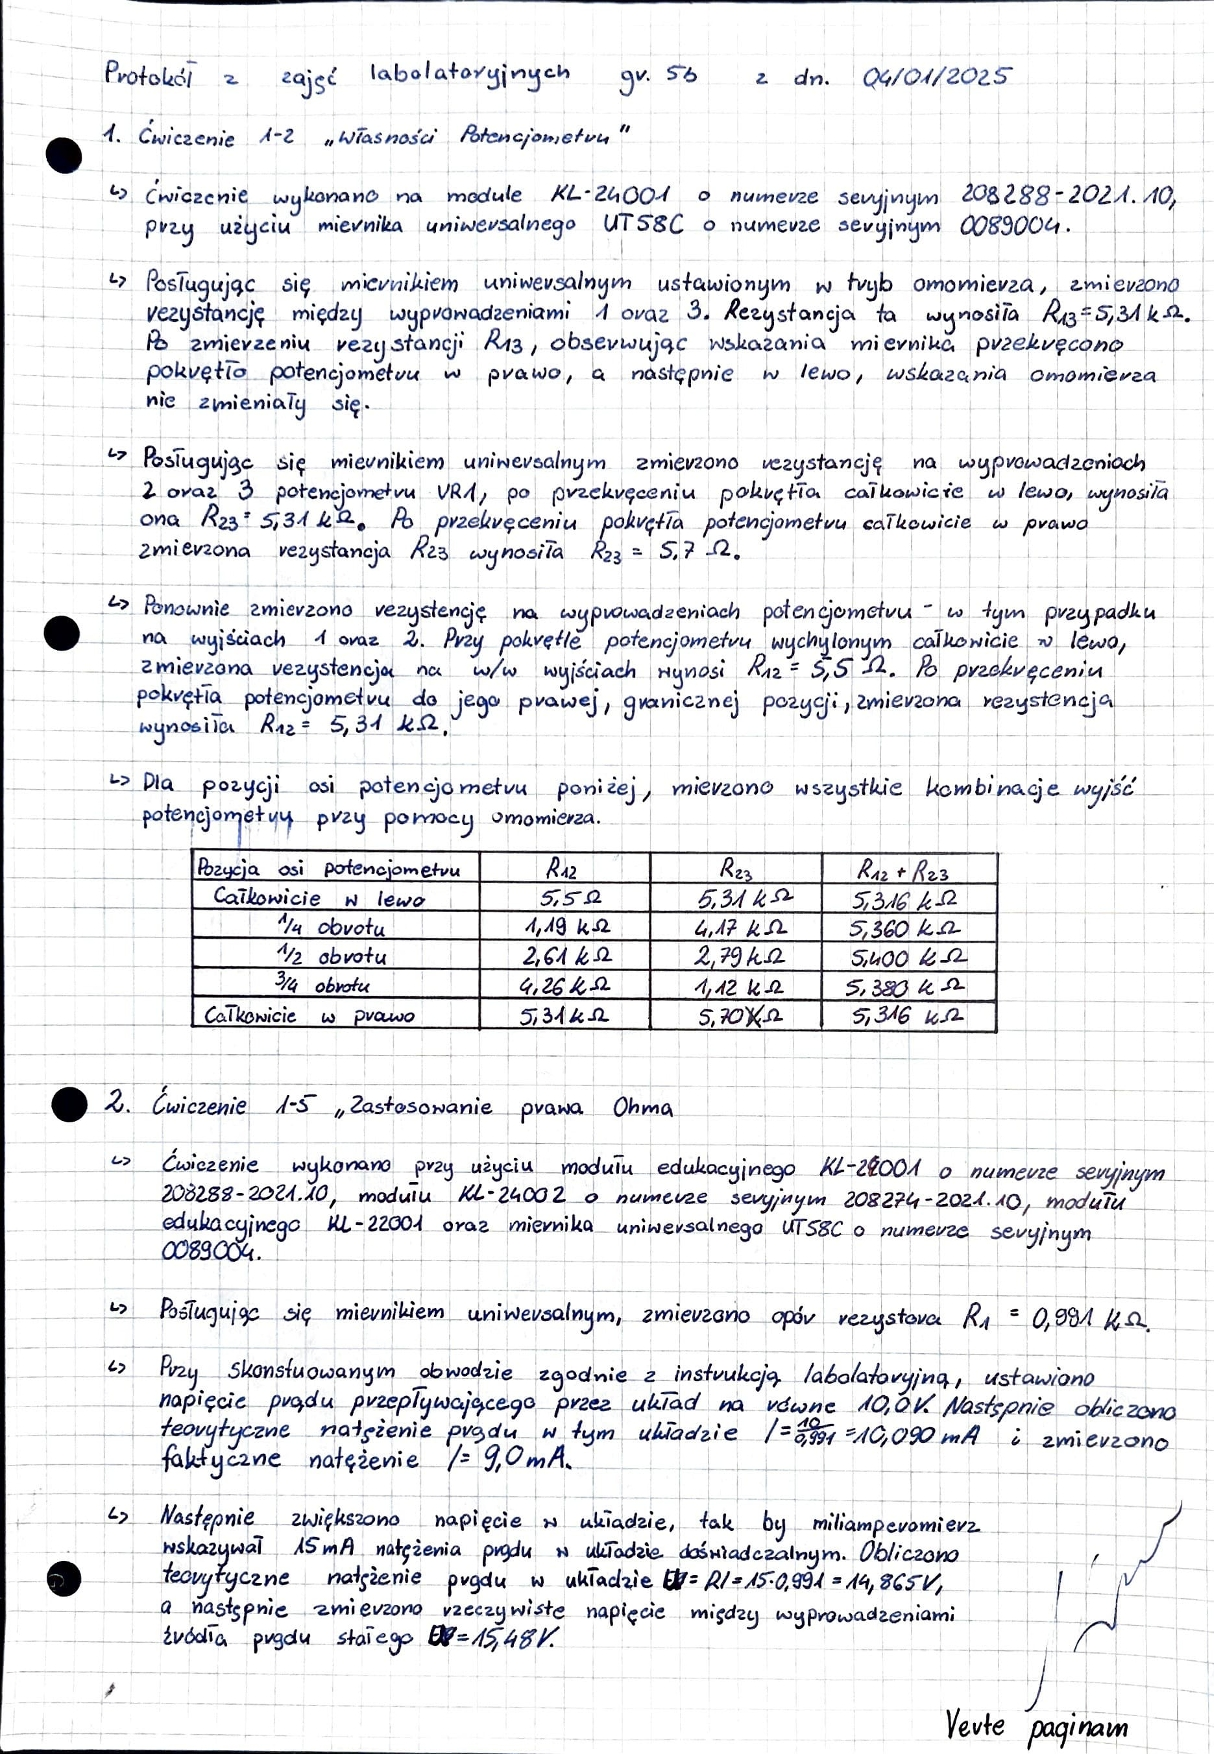
\includegraphics[height=0.95\textheight, width= \linewidth]{Adobe Scan 16 sty 2025 (1)-1.jpg}\newpage
    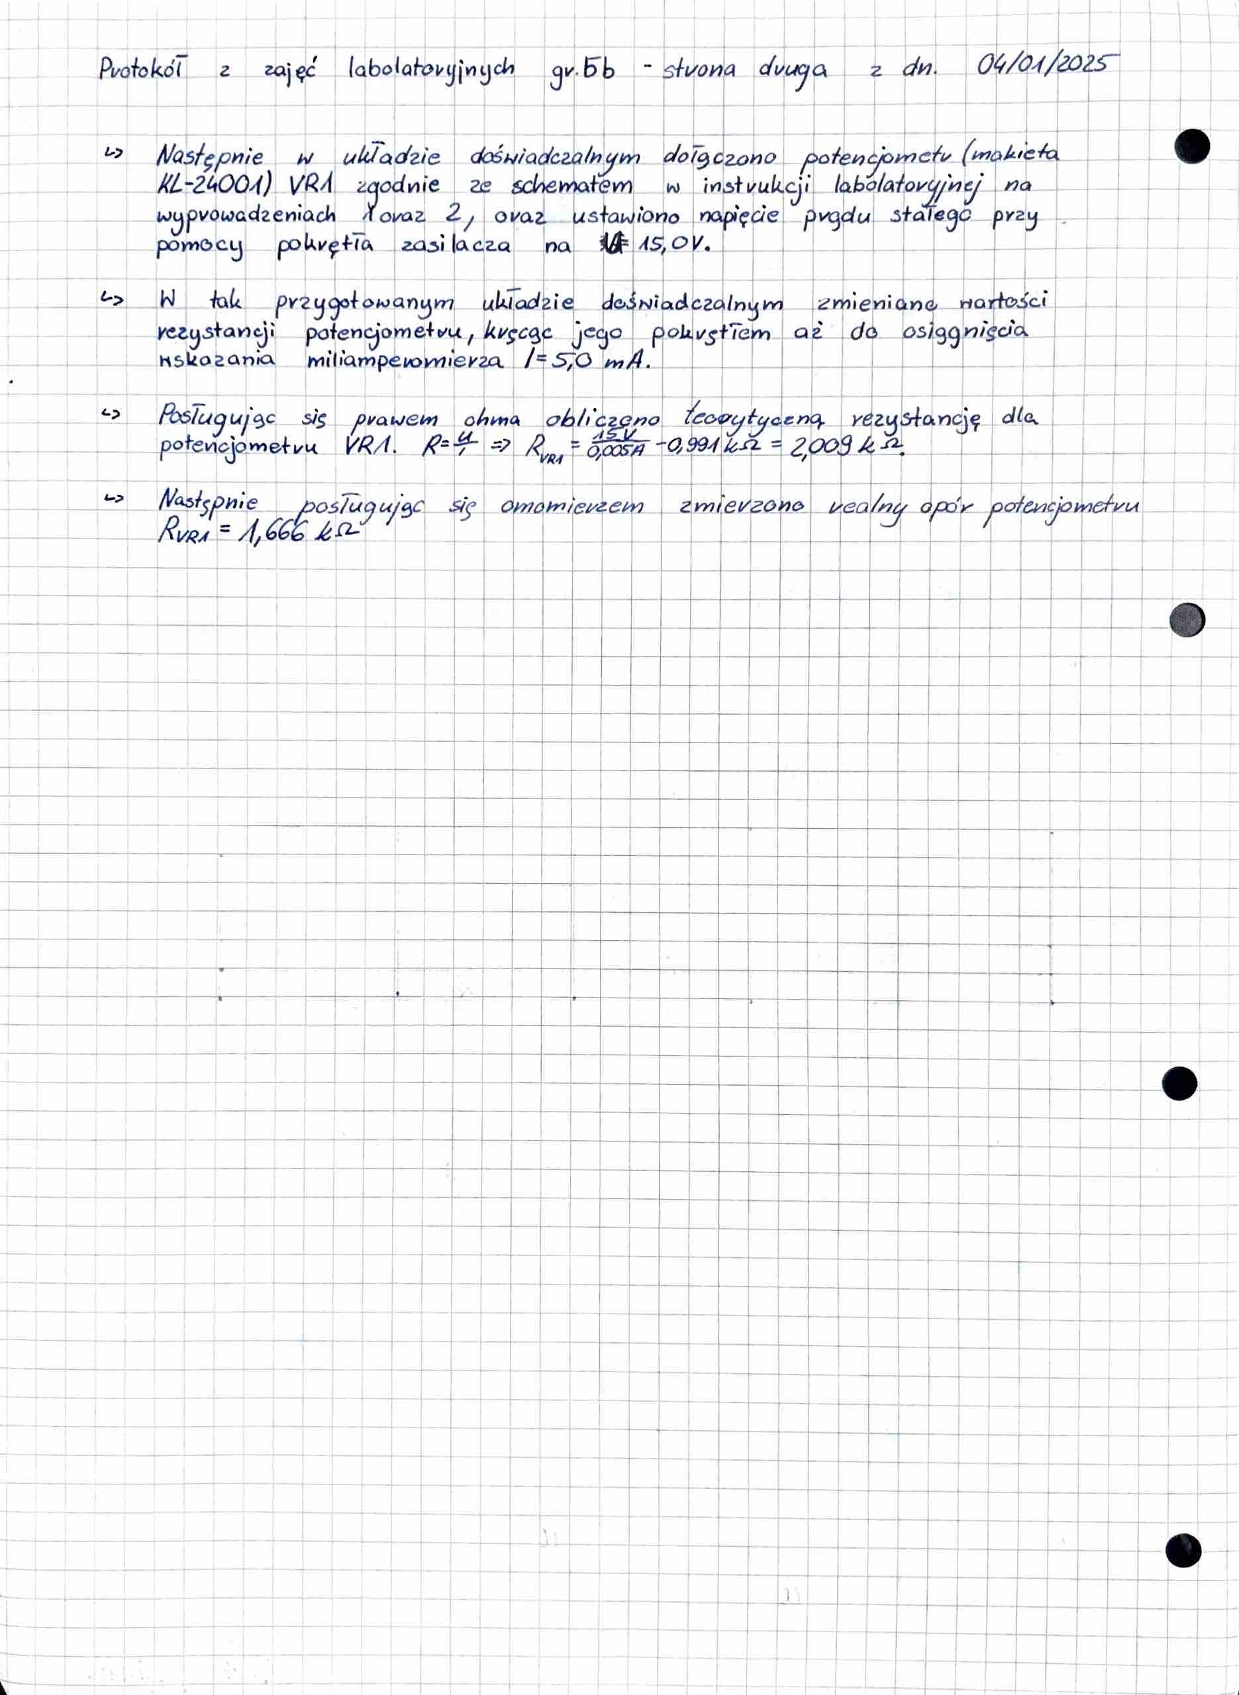
\includegraphics[height=\textheight, width= \linewidth]{Adobe Scan 16 sty 2025 (1)-2.jpg}
    

\end{document}
